%-----------------------------------------------------------------------
% Functional Programming 4
% John O'Donnell, Wim Vanderbauwhede
% University of Glasgow
%-----------------------------------------------------------------------

\documentclass{beamer}
\usepackage{jtodlecseriesFP4}

% Identify this presentation
\SetPresentationTitle
  {Equational Reasoning}
  {Equational Reasoning}
\SetPresentationNumber
  {6}
\SetPresentationDate
  {Week 3-3 (optional)}
  {Week 3-3 (optional)}

%-----------------------------------------------------------------------

% Beginning

\begin{document}

\begin{frame}
  \PresentationTitleSlide
\end{frame}


%-----------------------------------------------------------------------

\begin{frame}
  \frametitle{Topics}
  \tableofcontents
\end{frame}
%-----------------------------------------------------------------------
\section{Equational Reasoning}
\begin{frame}
\begin{center}
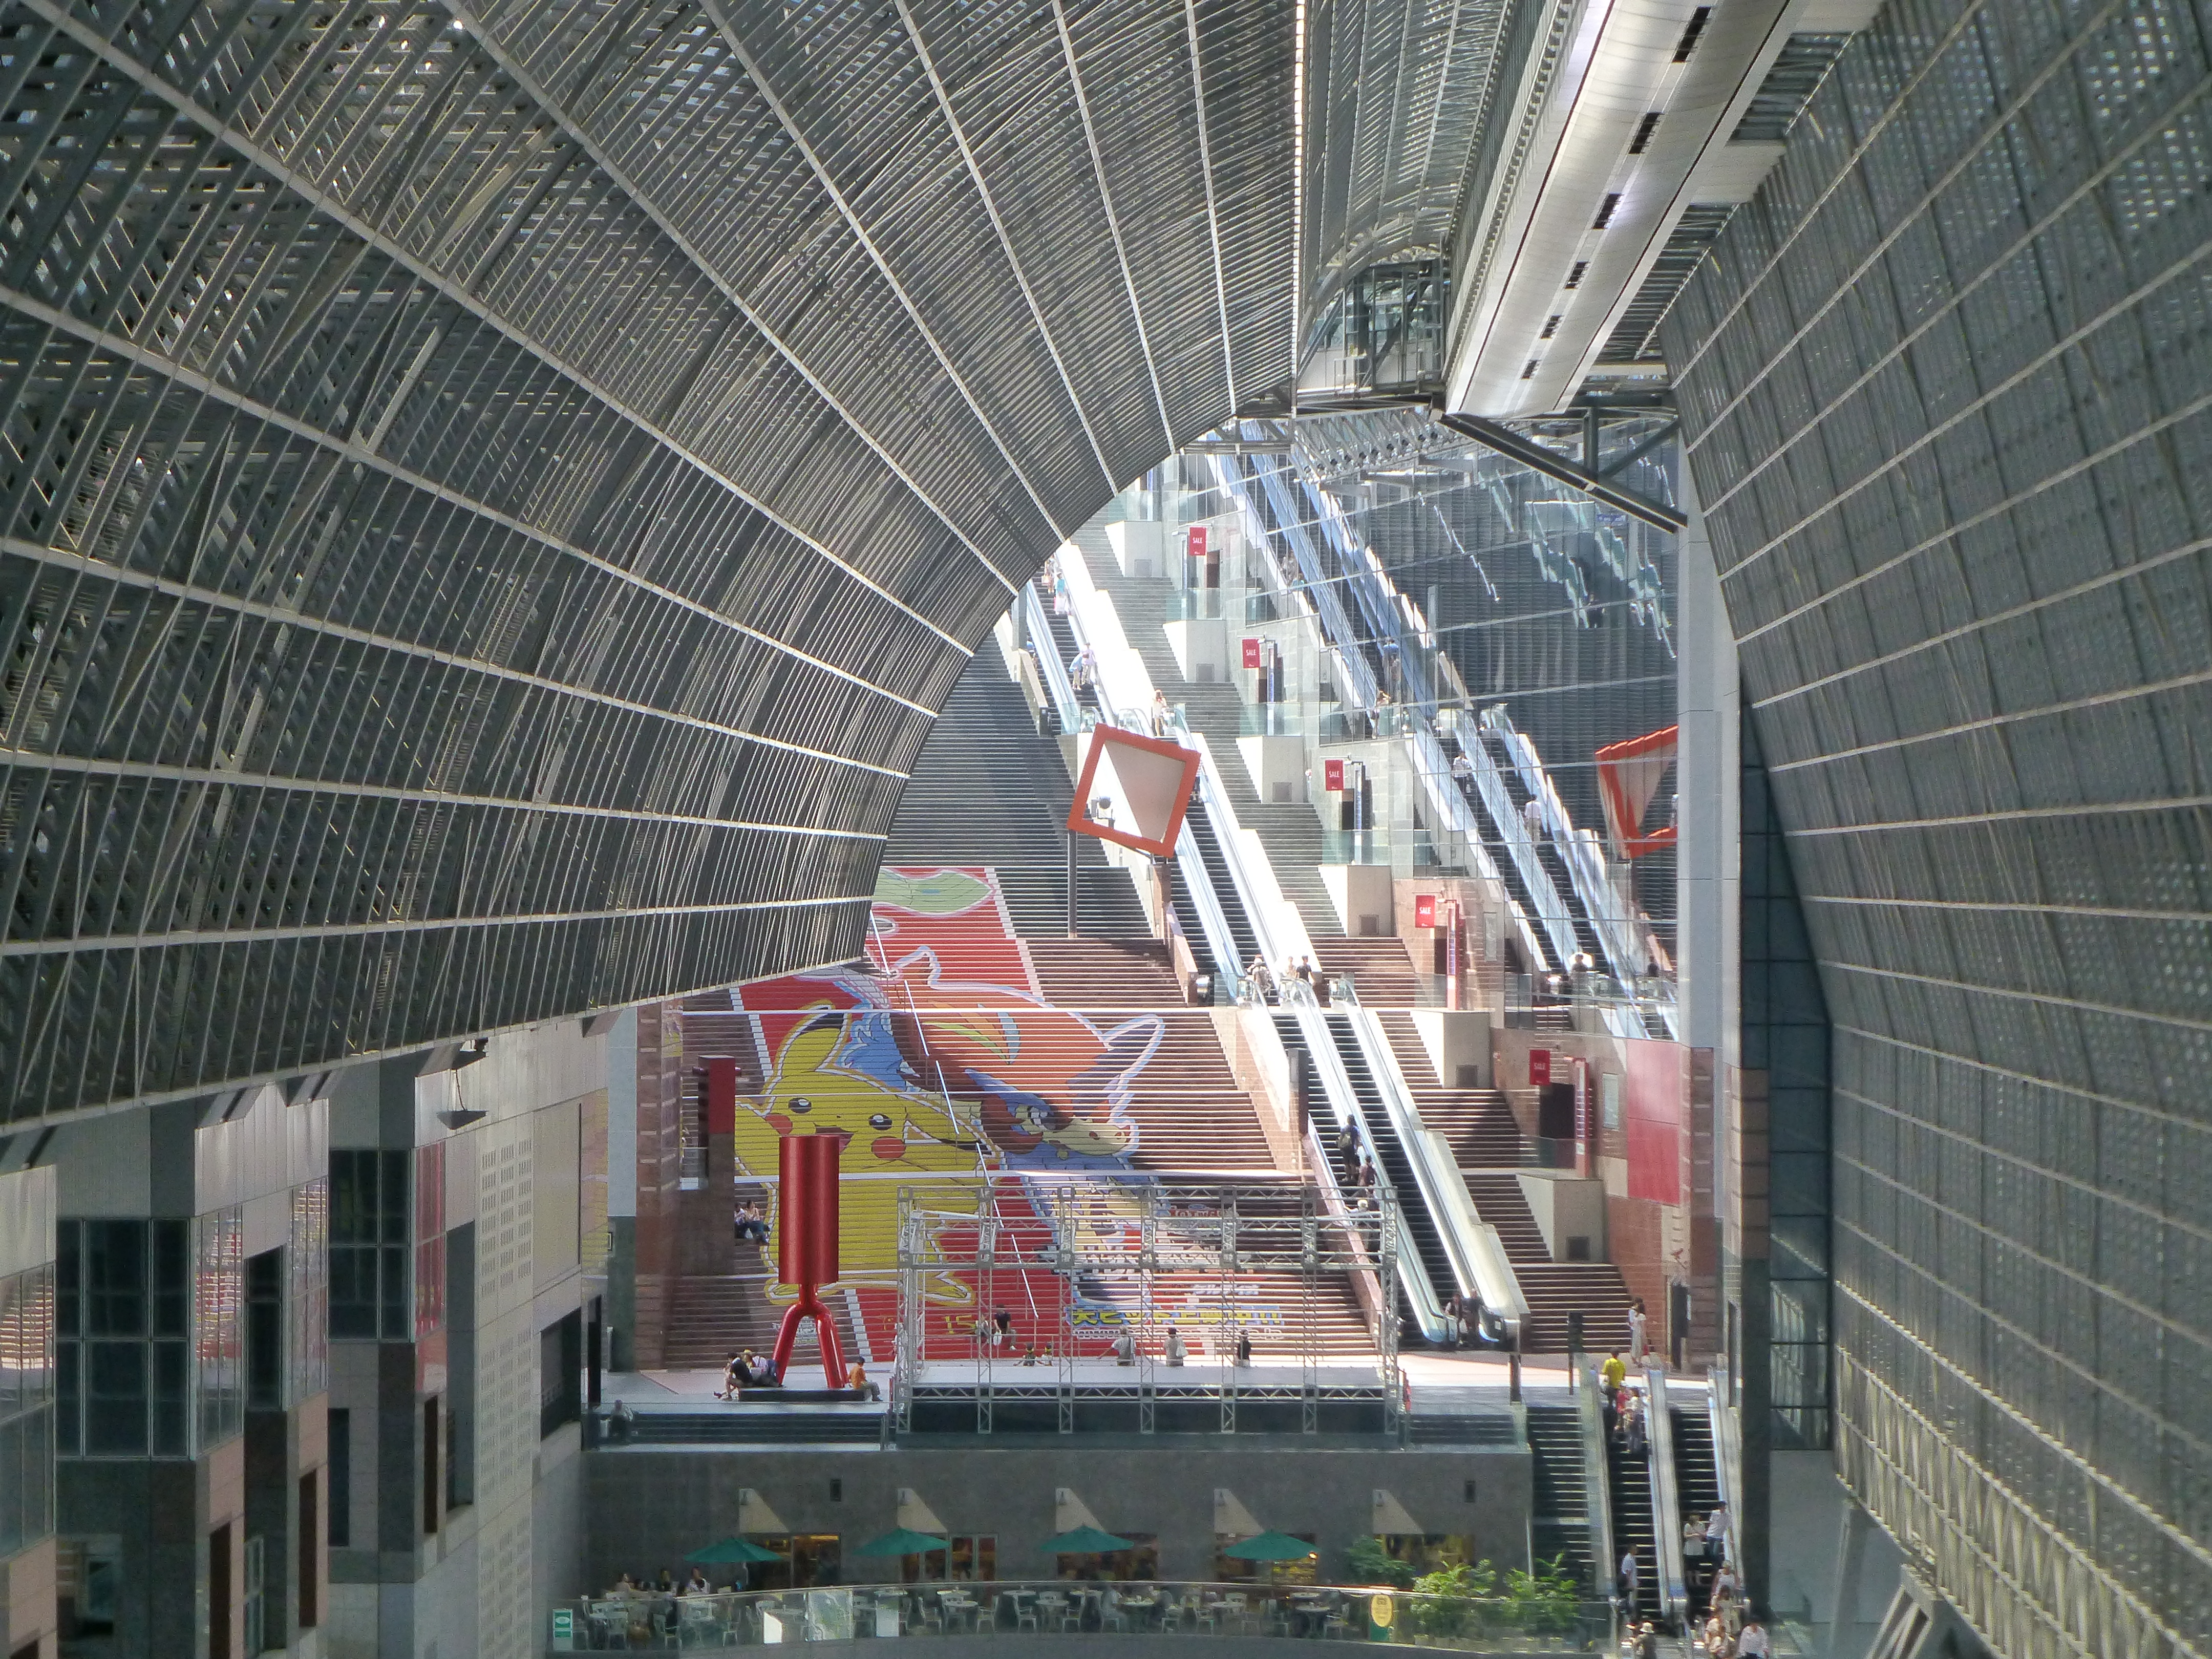
\includegraphics[scale=0.075]
    {figures/jpg/pic06b.jpg}
\end{center}
\end{frame}

%-----------------------------------------------------------------------

%-----------------------------------------------------------------------

\begin{frame}[fragile]
\frametitle{Equational reasoning}

\begin{itemize}
\item One of the greatest advantages of pure functional programming
  is that it works well with \emph{formal methods}
\item You can use formal methods to
  \begin{itemize}
  \item Prove correctness of a program
  \item Transform a program to improve its efficiency (the compiler
    does this extensively)
  \item Derive a program from a specification
  \end{itemize}
\item The most important kind of formal method in a pure language
  is \emph{equational reasoning}
\item This means ``substituting equals for equals'', taking
  advantage of the facts that $=$ really means mathematical
  equality, and there are no side effects.
\end{itemize}

\end{frame}

%-----------------------------------------------------------------------
\begin{frame}[fragile]
\frametitle{Definitions}

Here are some definitions we've already seen.  Each is annotated
with an equation name

\begin{verbatim}
map :: (a->b) -> [a] -> [b]          { map/type }
map f [] = []                        { map/1 }
map f (x:xs) = f x : map f xs        { map/2 }
\end{verbatim}

\begin{verbatim}
(.) :: (b->c) -> (a->b) -> a -> c   { (.)/type }
(f.g) x = f (g x)                   { (.) }
\end{verbatim}
\end{frame}

%-----------------------------------------------------------------------
\begin{frame}[fragile]
\frametitle{The map/compose theorem}

This theorem says that two traversals over a list, in order to
apply $g$ and then $f$ to each element, can be replaced by a single
traversal that applies the composition $f.g$

\begin{theorem}
  Let $g :: a->b$ and $f :: b->c$.  Then for any finite list $xs ::
  [a]$,
\begin{verbatim}
map f (map g xs) = map (f.g) xs
\end{verbatim}
\end{theorem}

This is a simple and elegant piece of mathematics, and it also
leads to some major optimisations in the Haskell compiler.

\end{frame}

%-----------------------------------------------------------------------
\begin{frame}[fragile]
\frametitle{Proof}

Proof by induction over $xs$.  We perform the proof by pure
algebra, using the code that defines the functions (this code
consists of mathematical equations).

Base case.

\begin{verbatim}
   map f (map g [])
= { map/1 }
   map f []
= { map/1 }
   []
= { map/1 }
   map (f.g) []
\end{verbatim}

\end{frame}

%-----------------------------------------------------------------------
\begin{frame}[fragile]
\frametitle{Induction case}

Induction case.  Assume the induction hypothesis: $map f (map g xs)
= map (f.g) xs$.  The aim is to prove $map f (map g (x:xs)) = map
(f.g) (x:xs)$.

\begin{verbatim}
  map f (map g (x:xs))
= { map/2 }
  map f (g x : map g xs)
= { map/2 }
  f (g x) : map f (map g xs)
= { induction hypothesis }
  f (g x) : map (f.g) xs
= { (.) }
(f.g) x : map (f.g) xs
= { map.2 }
  map (f.g) (x:xs)
\end{verbatim}

\end{frame}

%-----------------------------------------------------------------------
\begin{frame}[fragile]
\frametitle{Some observations}

\begin{itemize}
\item Sometimes formal methods are applied to a ``formalisation''
  of a program.  The resulting proofs apply to the formalisation,
  \emph{not to the actual software}.
\item We have proved the theorem \emph{using the actual Haskell
    source code}.  The theorem \emph{guarantees a property of the
    actual software}. This holds for LiveScript too.
\item The proof exploits the fact that there are no side effects.
\item There are some technical issues.  The most important is that
  we have proved that the theorem holds for all well typed finite
  lists.
\item Haskell also has infinite lists.  The theorem is valid for
  those too, but a more powerful proof technique is required for
  theorems about infinite data structures.
\end{itemize}

\end{frame}

%-----------------------------------------------------------------------
%\section{Lambdas Everywhere}
%\begin{frame}[fragile]
%\frametitle{Lambda Functions}
%\end{frame}
%
%%-----------------------------------------------------------------------
%
%\begin{frame}[fragile]
%\frametitle{Lambdas Everywhere}
%\begin{itemize}
%\item Lists are lambdas
%\item Tuples are lambdas
%\end{itemize}
%
%\end{frame}
\end{document}
